\documentclass{article}

\usepackage[english, russian]{babel}
\usepackage{geometry}
\usepackage{graphicx}
\usepackage{listings}
\usepackage{xcolor}
\usepackage[14pt]{extsizes}
\usepackage{amsmath}
\usepackage{setspace}
\usepackage{multirow}
\usepackage{tocloft}
\usepackage{indentfirst} 
\usepackage{lipsum}
\usepackage{caption}
\usepackage{cmap}
\usepackage[utf8]{inputenc}
\usepackage[T2A]{fontenc}

\captionsetup[figure]{name={Рисунок},labelsep=endash}
\captionsetup[table]{singlelinecheck=false, labelsep=endash}

\renewcommand{\cftsecleader}{\cftdotfill{\cftdotsep}}
\geometry{pdftex, left = 3cm, right = 1cm	, top = 2cm, bottom = 2cm}
\onehalfspacing

\setlength{\parindent}{1,25cm}
\lstdefinestyle{python}{
	language={Python},
	basicstyle=\footnotesize\ttfamily,
	frame=single,
	tabsize=4,	
	breaklines=true
}

\DeclareCaptionLabelSeparator{line}{\ --\ }
\DeclareCaptionFont{white}{\color{white}}
\DeclareCaptionFormat{listing}{\colorbox[cmyk]{0.43,0.35,0.35,0.01}{\parbox{\textwidth}{\hspace{15pt}#1#2#3}}}
\captionsetup[lstlisting]{
	singlelinecheck=false,
	labelsep=line
}

\begin{document}
\begin{titlepage}
	\newgeometry{pdftex, left=2cm, right=2cm, top=2.5cm, bottom=2.5cm}
	\fontsize{12pt}{12pt}\selectfont
	\noindent\begin{tabular}{|c|c|}	\hline
	\noindent\begin{minipage}{0.15\textwidth}
		
\includegraphics[width=\linewidth]{tools/logo.png}
	\end{minipage} &
	\noindent\begin{minipage}{0.85\textwidth}\centering
		\textbf{\newline Министерство науки и высшего образования Российской Федерации}\\
		\textbf{Федеральное государственное бюджетное образовательное учреждение высшего образования}\\
		\textbf{«Московский государственный технический университет имени Н.Э.~Баумана}\\
		\textbf{(национальный исследовательский университет)»}\\
		\textbf{(МГТУ им. Н.Э.~Баумана)}
	\end{minipage} \\
	\hline	\end{tabular}\newline\newline\newline
	\noindent ФАКУЛЬТЕТ \underline{«Информатика и системы управления»} \newline\newline
	\noindent КАФЕДРА \underline{«Программное обеспечение ЭВМ и информационные технологии»}\newline\newline\newline\newline\newline\newline

	\noindent\begin{minipage}{1.0\textwidth}\centering
		\Large\textbf{   ~~~ Лабораторная работа №1}\newline
		\textbf{по дисциплине «Архитектура ЭВМ»}\newline\newline\newline\newline\newline
	\end{minipage}

	\noindent\textbf{Тема} \underline{Проектирование систем на кристалле на основе ПЛИС}\newline\newline
	\textbf{Студент} \underline{Тузов Даниил Александрович}\newline\newline
	\textbf{Группа} \underline{ИУ7-52Б}\newline\newline
	\textbf{Преподаватель} \underline{Калитвенец Максим, Попов А.Ю.}
	
	\begin{center}
		\vfill
		Москва, \the\year ~г.
	\end{center}
	\restoregeometry
	\clearpage
\end{titlepage}

\textbf{Цель работы --} изучение основ построения микропроцессорных систем на ПЛИС. 
Для достижения поставленной цели необходимо решить следующие задачи:
\begin{itemize}
	\item[--] ознакомиться с принципами построения систем на кристалле (СНК) на основе ПЛИС;
	\item[--] получить навыки проектирования СНК в САПР Altera Quartus II;
	\item[--] выполнить проектирование и верификацию системы с использованием отладочного  комплекта Altera 
	DE1Board.
\end{itemize}

На рисунке \ref{fscheme} приведена функциональная схема разрабатываемой системы на кристалле.

\begin{figure}[h]
	\centering
	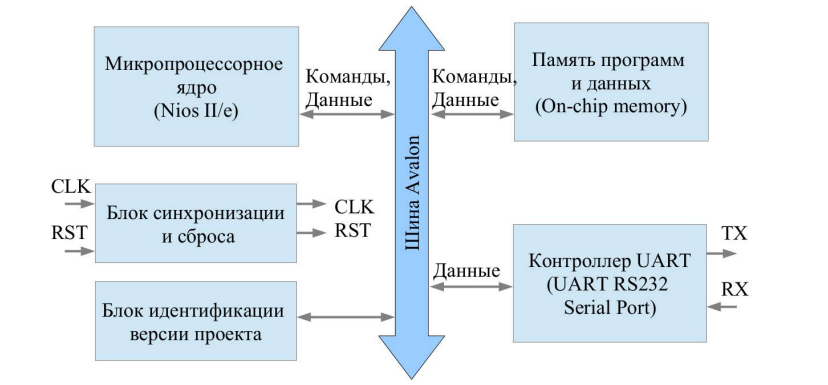
\includegraphics[scale=1]{tools/func_scheme.png}
	\caption{Функциональная схема разрабатываемой системы на кристалле}
	\label{fscheme}
\end{figure}

\section{Введение}
Система на кристалле, приведенная на рисунке \ref{fsheme} состоит из следующих блоков:
\begin{itemize}
	\item[--] микропроцессорное ядро Nios II/e выполняет функции управления системой;
	\item[--] внутренняя оперативная память СНК, используемая для хранения программы управления и данных;
	\item[--] системная шина Avalon обеспечивает связность всех компонентов системы;
	\item[--] блок синхронизации и сброса обеспечивает обработку входных сигналов сброса и синхронизации и 
распределение их в системе. Внутренний сигнал сброса синхронизирован и имеет необходимую для системы 
длительность;
	\item[--] блок идентификации версии проекта обеспечивает хранение и выдачу уникального идентификатора 
версии, который используется программой управления при инициализации системы;
	\item[--] контроллер UART обеспечивает прием и передачу информации по интерфейсу RS232.
\end{itemize}

\clearpage\section{Настройки}
В ходе выполнения лабораторной работы, были выполнены соответствующие настройки, приведенные на рисунках
\ref{qsys} -- \ref{view}.

\begin{figure}[h]
	\centering
	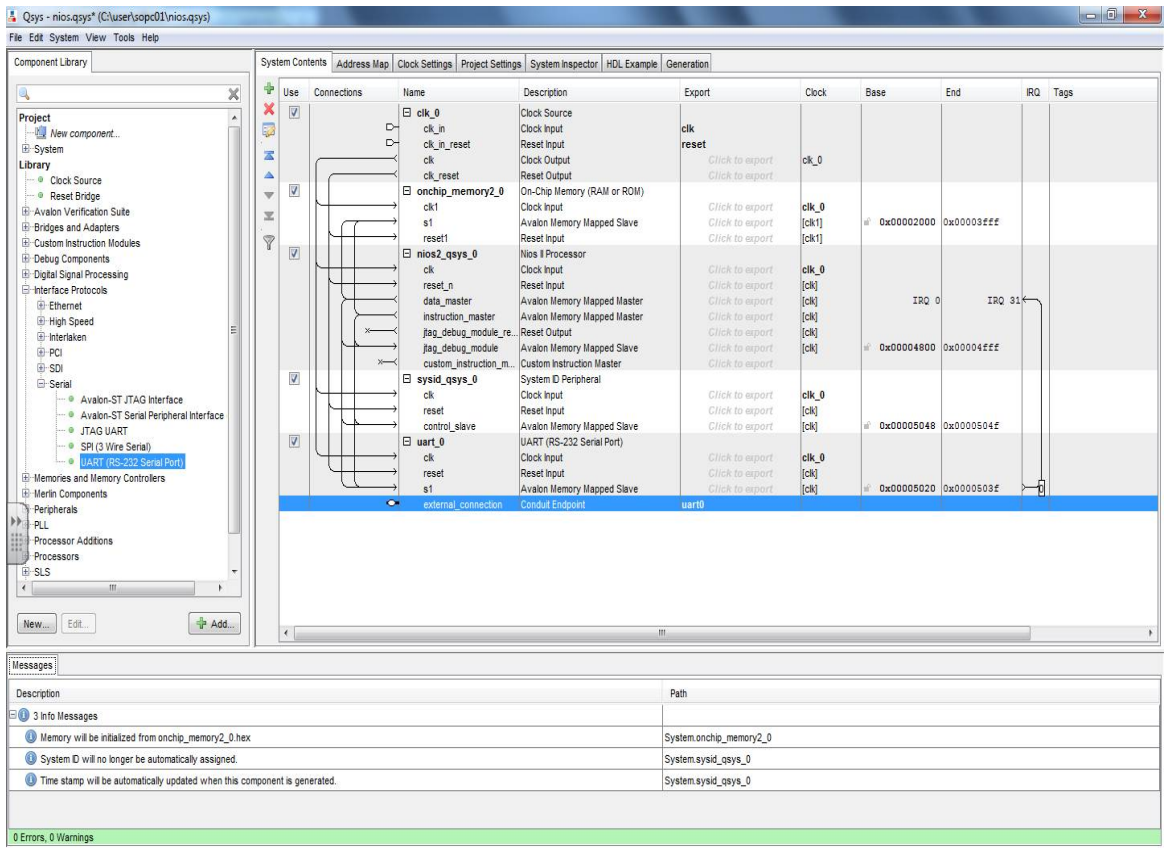
\includegraphics[scale=0.7]{tools/qsys.png}
	\caption{Готовый модуль в системе проектирования систем на кристалле Altera Qsys}
	\label{qsys}
\end{figure}

\begin{figure}[h]
	\centering
	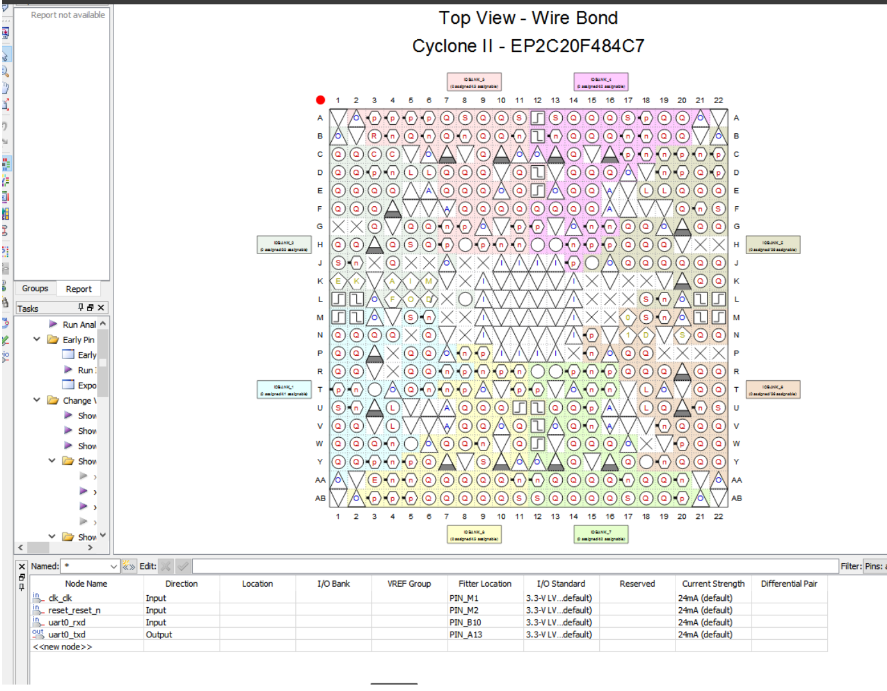
\includegraphics[scale=0.8]{tools/view.png}
	\caption{Таблица распределение адресов модулей в системе на кристалле}
	\label{view}
\end{figure}

\clearpage\section{Разработанное ПО}
На рисунках \ref{echo} -- \ref{variant} приведен код программного проекта Nios II Software Build Tools for 
Eclipse.
\begin{figure}[h]
	\centering
	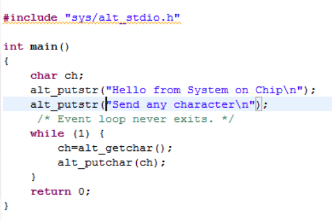
\includegraphics[scale=1]{tools/echo.png}
	\caption{Программа эхо}
	\label{echo}
\end{figure}

\begin{figure}[h]
	\centering
	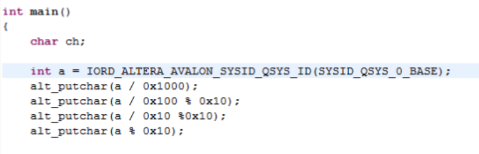
\includegraphics[scale=1]{tools/variant.png}
	\caption{Программа, выполняющая вывод номера варианта}
	\label{variant}
\end{figure}

\clearpage\section{Тестирование}
На рисунке \ref{verif} приведен результат работы программы, представленной на рисунке \ref{variant}.
\begin{figure}[h]
	\centering
	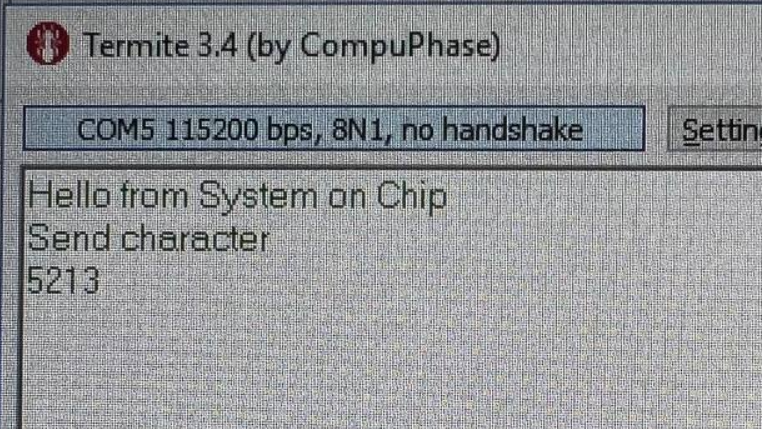
\includegraphics[scale=1]{tools/verif.png}
	\caption{Результат работы программы}
	\label{verif}
\end{figure}

\end{document}